\documentclass[tikz,border=2mm]{standalone}
\usepackage[T1]{fontenc}
\usepackage{lmodern}
\usetikzlibrary{arrows.meta,positioning,fit,calc}

\definecolor{principle}{HTML}{DCEAF7}
\definecolor{evidence}{HTML}{E2F0DC}
\definecolor{policy}{HTML}{F5E0B8}
\definecolor{limit}{HTML}{F2D6D6}

\begin{document}
\sffamily
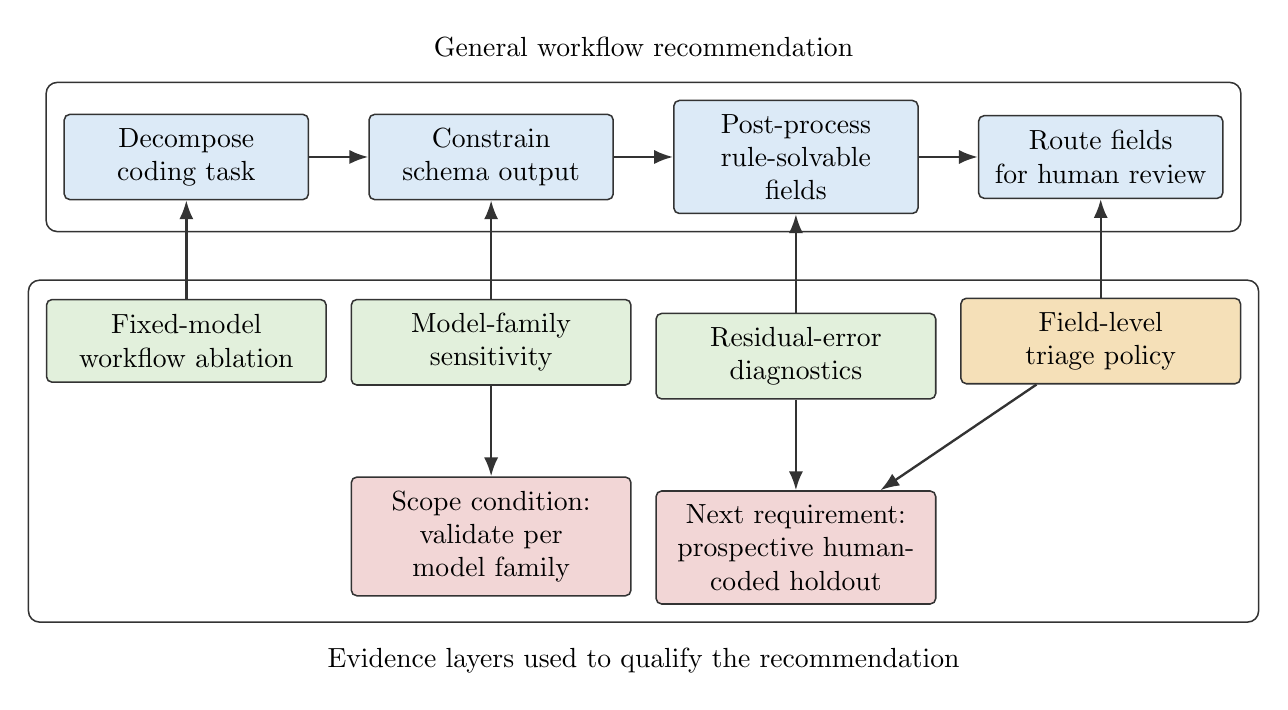
\begin{tikzpicture}[
  >=Latex,
  line/.style={draw=black!80, line width=0.55pt},
  arrow/.style={-Latex, draw=black!80, line width=0.85pt},
  box/.style={line, rounded corners=2pt, minimum height=1.05cm, text width=2.75cm, align=center, inner sep=5pt, font=\normalsize},
  widebox/.style={line, rounded corners=2pt, minimum height=1.05cm, text width=3.2cm, align=center, inner sep=5pt, font=\normalsize},
  note/.style={align=center, font=\normalsize}
]

\node[box, fill=principle] (decompose) {Decompose\\coding task};
\node[box, fill=principle, right=0.75cm of decompose] (constrain) {Constrain\\schema output};
\node[box, fill=principle, right=0.75cm of constrain] (rules) {Post-process\\rule-solvable fields};
\node[box, fill=principle, right=0.75cm of rules] (review) {Route fields\\for human review};

\draw[arrow] (decompose) -- (constrain);
\draw[arrow] (constrain) -- (rules);
\draw[arrow] (rules) -- (review);

\node[widebox, fill=evidence, below=1.25cm of decompose] (fixed) {Fixed-model\\workflow ablation};
\node[widebox, fill=evidence, below=1.25cm of constrain] (families) {Model-family\\sensitivity};
\node[widebox, fill=evidence, below=1.25cm of rules] (diagnostic) {Residual-error\\diagnostics};
\node[widebox, fill=policy, below=1.25cm of review] (triage) {Field-level\\triage policy};

\draw[arrow] (fixed) -- (decompose);
\draw[arrow] (families) -- (constrain);
\draw[arrow] (diagnostic) -- (rules);
\draw[arrow] (triage) -- (review);

\node[widebox, fill=limit, below=1.15cm of families] (scope) {Scope condition:\\validate per model family};
\node[widebox, fill=limit, below=1.15cm of diagnostic] (holdout) {Next requirement:\\prospective human-coded holdout};

\draw[arrow] (families) -- (scope);
\draw[arrow] (diagnostic) -- (holdout);
\draw[arrow] (triage) -- (holdout);

\node[line, rounded corners=4pt, fit=(decompose)(constrain)(rules)(review), inner sep=0.22cm] (principlefit) {};
\node[note, above=0.20cm of principlefit.north] {General workflow recommendation};

\node[line, rounded corners=4pt, fit=(fixed)(families)(diagnostic)(triage)(scope)(holdout), inner sep=0.22cm] (evidencefit) {};
\node[note, below=0.20cm of evidencefit.south] {Evidence layers used to qualify the recommendation};

\end{tikzpicture}
\end{document}
